% OODA-Aegis, IEEE two-column layout (same text as ooda_aegis_preprint.tex). Build: tectonic ooda_aegis_ieee.tex
\documentclass[journal]{IEEEtran}
\usepackage[T1]{fontenc}
\usepackage{amsmath}
\usepackage{newtxtext,newtxmath}
\usepackage{microtype}
\usepackage{booktabs}
\usepackage{graphicx}
\usepackage{xcolor}
\usepackage{adjustbox}
\usepackage[hidelinks]{hyperref}
\setcounter{dbltopnumber}{4}
\renewcommand{\dbltopfraction}{0.92}
\renewcommand{\dblfloatpagefraction}{0.75}
\renewcommand{\textfraction}{0.08}
\newcommand{\phisafe}{\ensuremath{\Phi_{\mathrm{safety}}}}
\newcommand{\code}[1]{\texttt{#1}}
\newcommand{\repolink}{\url{https://github.com/CopyNinja07-07/aegis}}

\title{OODA-Aegis: Exploit-Grounded, Constraint-Verified Program Repair with Code-Graph Retrieval and SMT Guardrails}
\author{Nikhil Kumar and Suryansh Pratap Singh%
\thanks{Nikhil Kumar is the lead author. Manuscript finalized November 2026. Code, benchmark, raw logs and notebooks: \repolink{}.}}

\begin{document}
\maketitle

\begin{abstract}
Small open models can write security patches, but nothing they produce can be trusted on its own: the repair model's own test agreed with an independent verifier on only 56\% of candidate fixes. OODA-Aegis, built on Boyd's Observe--Orient--Decide--Act loop, treats every Gemma 4 output as an untrusted proposal: a static call graph retrieves the code around the attacked route, the Z3 SMT solver checks every edge rule and patch, and an agent-built gate accepts a patch only if the exploit worked before it, fails after it, and legitimate requests get the same responses. On AegisBench, 16 executable repair tasks in 9 vulnerability classes run on free Kaggle T4 GPUs, the agent verified 45 of 48 fixes; the route file alone gave 0 of 32, trusting the model's own test shipped broken patches, and E4B matched 31B at four times the speed. With bugs up to five call hops away, the call slice verified 27 of 32 fixes against 15 for the whole repository ($p = 0.003$), while a 2-hop limit passed the gate only by guarding an outer layer, which a dynamic-taint clause rejects without a reference fix. On 13 real CVEs with reproducing exploits (up to 151k lines), graph plus exploit trace reaches every bug and works best as a filter for similarity ranking; on CVE-2021-33503 the verified patches were mitigations, not the upstream fix. Simple injections never changed the model's actions.
\end{abstract}

\begin{IEEEkeywords}
Agentic software engineering, automated program repair, code-graph retrieval, SMT verification, Gemma 4, vulnerability repair, benchmarks.
\end{IEEEkeywords}

\section{Introduction}

Coding agents such as SWE-agent~\cite{sweagent} follow generate-and-validate repair~\cite{genprog,monperrus}: propose a change, keep it if tests pass. For security fixes this breaks three ways: the patch author's own test shares its blind spots~\cite{overfit}; model-written filters miss encoded attacks and rewrites break legitimate behaviour; and the bug sits in code the handler calls, which the handler hides and the whole repository buries.

OODA-Aegis keeps generation and verification apart: the model proposes; deterministic oracles, a code graph, a solver and a gate decide what runs. We frame Boyd's loop~\cite{boyd} as a constrained POMDP~\cite{altman} and evaluate it on Gemma 4 models that fit on one accelerator.

\paragraph{Contributions}
\begin{itemize}
\item \textbf{AegisBench}: 16 executable repair tasks with outcome oracles, legitimate-traffic checks and held-out variants. \textbf{AegisBench-Deep} moves each bug up to five call hops away.
\item \textbf{Code-graph retrieval} from Python's AST, tested across bug depths, dynamic, decorator and ORM indirection, and 13 real CVEs against similarity retrieval.
\item \textbf{Solver-checked actions}: Z3 proves edge rules cannot match protected requests and checks patches against named safety clauses; dynamic-taint and static no-bypass clauses test for root-cause fixes and bypasses.
\item \textbf{400 Kaggle episodes} (ablations, model sizes, injections, replays), 96 local deep episodes and 11 real-CVE trials, plus 694 gate-labelled repair attempts.
\end{itemize}

\paragraph{Findings}
\textbf{(F1)} Localisation is the bottleneck: the same model goes from 0/32 to 45/48 verified fixes when it sees the code the call graph selects; with the bug out of view it passes the gate only by guarding an outer layer. \textbf{(F2)} A model-written test approved 25 broken patches and rejected 59 correct ones. \textbf{(F3)} Inside a verifying loop, Gemma 4 E4B is as reliable as 31B and four times faster. \textbf{(F4)} Most of the gain from multi-candidate search pays for one formatting error. \textbf{(F5)} Simple, static injections did not change Gemma 4's actions; adaptive attacks are untested.

\paragraph{Track topics} \emph{Code Comprehension} (\S\ref{sec:orient}, \S\ref{sec:graph}, \S\ref{sec:cve}), \emph{Tasks \& Benchmarks} (\S\ref{sec:bench}), labelled data for \emph{Tuning \& Optimization} (\S\ref{sec:disc}), and an application (\S\ref{sec:app}).

\section{Problem formulation and threat model}

\subsection{Constrained POMDP}
We model incident response as a constrained POMDP $\langle S, A, T, R, \Omega, O, \phisafe \rangle$ with hidden state $s = (C, K, V)$ (code, attacker capability, vulnerabilities), observations $o = (y, \Delta t, \rho)$ (response, latency, redirect target) and actions $a = (a_{\mathrm{edge}}, a_{\mathrm{patch}})$ (a proxy filter, a source change).
\begin{itemize}
\item \textbf{Safety predicate, level 1 (edge actions, string theory).} No protected request may match the rule:
\begin{equation}
L(E_{\mathrm{rule}}) \cap R_{\mathrm{protected}} = \emptyset,
\end{equation}
where $E_{\mathrm{rule}}$ is the rule's regular language over all URIs, encoded forms included, and $R_{\mathrm{protected}}$ the health check and recorded legitimate requests; Z3's string theory decides it exactly.
\item \textbf{Safety predicate, level 2 (patches, propositional).} Five named clauses over the diff $\Delta C$ from $C$ to $C'$, each a decidable syntactic fact computed from the AST:
\begin{equation}
\begin{split}
\phisafe(a_{\mathrm{patch}}) = {} & \underbrace{\mathrm{Files}(\Delta C) \subseteq \mathrm{Files}(N(f_0))}_{\mathit{in\_scope}}\\
& \wedge \underbrace{\mathrm{Sig}(C') \supseteq \mathrm{Sig}(C)}_{\mathit{api\_kept}} \wedge \mathit{protected\_kept}\\
& \wedge \mathit{no\_new\_sinks} \wedge \underbrace{\Delta C \neq \emptyset}_{\mathit{changed}}.
\end{split}
\end{equation}
Z3 only combines them and names a violated one through its UNSAT core; level 2 says nothing about what the patched code computes, which only the gate tests (\S\ref{sec:act}).
\end{itemize}
The model proposes $a \sim \pi_\theta(\cdot \mid o, G_{\mathrm{code}})$; no policy is learned. The agent executes the projection
\begin{equation}
a_{\mathrm{exec}} = P_{\phisafe}(a) =
\begin{cases}
a & \text{if Z3 proves } \phisafe(a),\\
\bot & \text{otherwise (escalate to a human).}
\end{cases}
\end{equation}

\subsection{Threat model}
The attacker controls request parameters and headers and can inject instructions via headers, leaked responses or repository comments. Oracles, graph builder, Z3 and gate are trusted; the models are not.

\section{The OODA-Aegis agent}

\begin{figure*}[!t]
\centering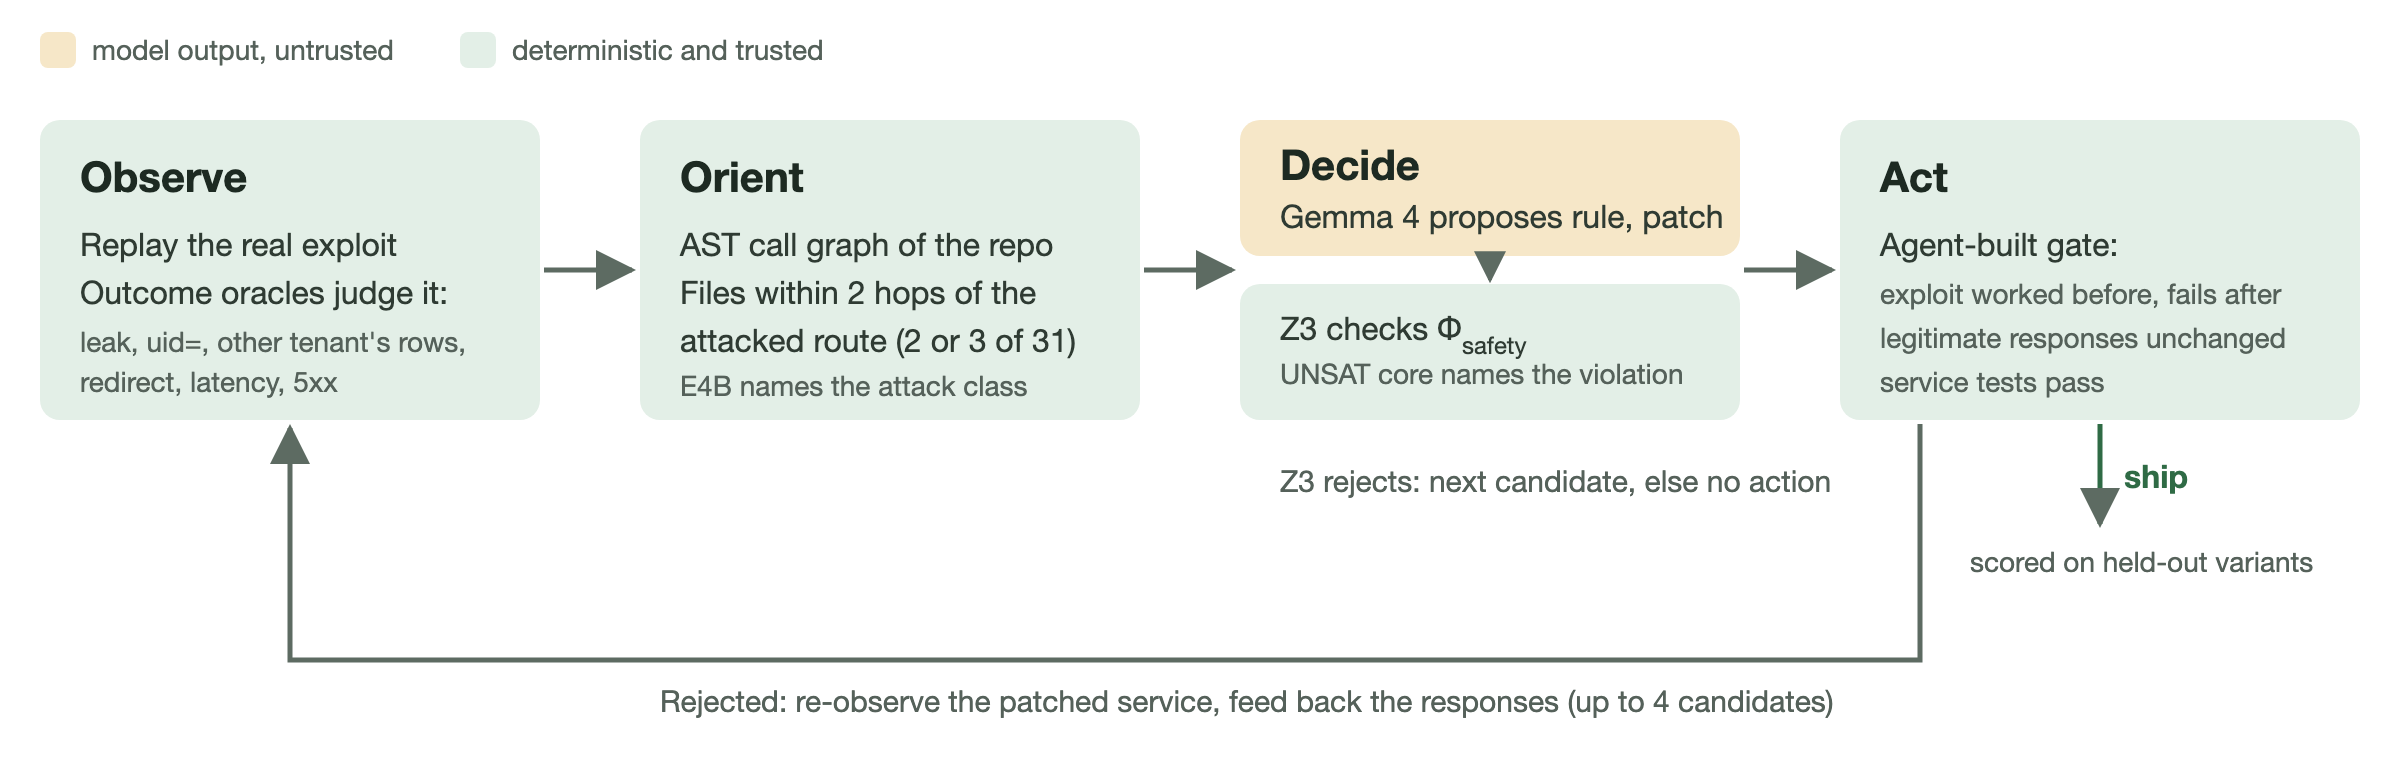
\includegraphics[width=\linewidth]{../fig_loop.png}
\caption{The OODA-Aegis loop. Amber marks model output (untrusted); green marks deterministic, trusted steps. A rejected patch sends the agent back to observe the patched service.}
\label{fig:loop}
\end{figure*}

\subsection{Observe: outcome oracles}
The agent replays the exploit and asks whether it \emph{worked}, not whether the input looks malicious:
\begin{equation}
\begin{split}
\mathcal{O}(r) \iff {} & \mathrm{Leak}(y) \vee \mathrm{CrossTenant}(y) \vee \mathrm{ExtRedirect}(\rho)\\
& \vee \Delta t > 1\,\mathrm{s} \vee \mathrm{status}(y) \geq 500,
\end{split}
\end{equation}
where $\mathrm{Leak}$ detects a password file, a canary token or command output (\code{uid=}).

\subsection{Orient: code graph and retrieval}\label{sec:orient}
A static call graph $G = (V, E)$ of functions and classes is built from the AST, resolving imports and attribute access; route decorators map each endpoint to its handler $f_0$. The repair context is every file containing a node within $k$ hops:
\begin{equation}
N_k(f_0) = \{ v \in V \mid d_G(f_0, v) \leq k \}.
\end{equation}
The main runs use $k = 2$; the forward call slice $N_\infty(f_0)$ takes every reachable function (\S\ref{sec:graph}). For dynamic calls the agent can add the calls $E_{\mathrm{trace}}$ recorded while replaying the legitimate requests, $G' = (V, E \cup E_{\mathrm{trace}})$, falling back from the static slice to $G'$ to the route file's import closure.

\subsection{Decide: solver-checked proposals}
\paragraph{Edge rules} To contain the attack, the edge model writes a rule in the language
\begin{equation}
\begin{split}
\mathcal{L}_{\mathrm{rule}} ::= {} & \mathtt{contains}(s_1, \dots, s_n) \mid \mathtt{max\_length}(n)\\
& \mid \mathtt{repeated\_run}(m),
\end{split}
\end{equation}
compiled to an encoding-aware proxy regex and a Z3 regular expression $E_{\mathrm{rule}}$; Z3 decides Eq.~1 (a counter-example is fed back), and the rule must also match the exploit.

\paragraph{Patches} The repair model states the invariant the code must enforce, then returns the patched file and its own pytest; AST facts are checked against Eq.~2, and a violated clause is named for feedback.

\subsection{Act: the agent-built gate and search}\label{sec:act}
A patch that passes Z3 is tested in a fresh copy of the repository. The gate requires that:
\begin{enumerate}
\item the exploit succeeds on the original code (the task is real);
\item the exploit and every visible variant are safe on the patched code, within 2.5\,s;
\item every recorded legitimate request returns the same status, redirect target and parsed JSON (key order, timing fields, UUID and timestamp values ignored);
\item the service's own tests pass.
\end{enumerate}
The model's own test is advisory. On rejection the agent feeds back the patched service's responses and samples again (temperature 0.2 or 0.8), up to $K = 4$ candidates. Accepted patches are scored on held-out variants never shown to the agent and labelled after the fact: with $\mathrm{Sink}$ the definitions the reference fix changes, a verified patch is
\begin{equation}
\mathrm{RootCause}(a_{\mathrm{patch}}) \iff \Delta C \cap \mathrm{Defs}(\mathrm{Sink}) \neq \emptyset,\label{eq:rootcause}
\end{equation}
and a \emph{path-specific guard} otherwise: the gate passed, but the vulnerable code is unchanged and reachable from other callers. As Eq.~\ref{eq:rootcause} needs a reference fix, we also test a clause the agent can check itself: replaying the exploit under a profiler marks the functions receiving the payload (dynamic taint); with $T_{\mathrm{sink}}$ those in the deepest one's module,
\begin{equation}
\mathit{sink\_changed}(a_{\mathrm{patch}}) \iff \Delta C \cap \big(T_{\mathrm{sink}} \cup \mathrm{Reads}(T_{\mathrm{sink}})\big) \neq \emptyset,\label{eq:taint}
\end{equation}
where $\mathrm{Reads}$ adds the module-level patterns and constants they read. A static clause, \emph{no\_sanitizer\_bypass}, rejects a patch if a parameter it adds reaches a sink (file, SQL text, shell string, HTTP request, deserialiser, format template, record lookup) before a validator of the original module or a raising check.

\section{AegisBench}\label{sec:bench}

AegisBench judges a fix by whether the attack still works and real users are unaffected. Its service, Vault, has 31 Python modules (430 lines).

\begin{enumerate}
\item \textbf{Bugs live in helpers.} Each task swaps one helper in \code{vault/core} for a vulnerable version (Table~\ref{tab:tasks}), one call hop from its route.
\item \textbf{Variants test generalisation.} Each task ships the exploit, 1 to 4 visible and 1 to 4 held-out variants (42 in total; the 31 that succeed against the vulnerable code are the ones scored).
\item \textbf{Naive fixes fail.} Each task records 2 or 3 legitimate requests: \code{deser-prefs} must keep loading legitimate pickles; \code{fmt-greet} must keep \code{\{user.name\}} working.
\end{enumerate}
A validation script checks that every exploit works and every reference fix passes the gate.

\begin{table*}[!t]
\centering\small
\caption{AegisBench tasks. Held-out variants never appear in the agent's prompts.}
\label{tab:tasks}
\begin{adjustbox}{max width=\linewidth}\begin{tabular}{lllcl}
\toprule
Task & Class & CWE & Variants (vis./held-out) & Vulnerable helper\\
\midrule
\code{pt-docs} & Path traversal & 22 & 4 / 4 & \code{storage.py} (\code{read\_blob})\\
\code{pt-templates} & Path traversal & 22 & 3 / 3 & \code{templates.py} (\code{load\_template})\\
\code{sqli-customers} & SQL injection & 89 & 3 / 3 & \code{db.py} (\code{find\_customer})\\
\code{sqli-notes} & SQL injection & 89 & 3 / 3 & \code{db.py} (\code{search\_notes})\\
\code{redos-email} & ReDoS & 1333 & 3 / 3 & \code{validate.py} (\code{is\_email})\\
\code{redos-slug} & ReDoS & 1333 & 3 / 3 & \code{validate.py} (\code{is\_slug})\\
\code{cmdi-status} & Command injection & 78 & 4 / 3 & \code{shell.py} (\code{echo\_status})\\
\code{cmdi-archive} & Command injection & 78 & 3 / 3 & \code{archive.py} (\code{list\_archive})\\
\code{ssrf-preview} & SSRF & 918 & 3 / 3 & \code{fetch.py} (\code{preview})\\
\code{ssrf-asset} & SSRF & 918 & 3 / 3 & \code{fetch.py} (\code{read\_asset})\\
\code{redirect-login} & Open redirect & 601 & 3 / 3 & \code{redirect.py} (\code{safe\_next})\\
\code{redirect-logout} & Open redirect & 601 & 3 / 3 & \code{redirect.py} (\code{logout\_target})\\
\code{idor-invoice} & IDOR & 639 & 2 / 1 & \code{billing.py} (\code{invoice\_for})\\
\code{idor-files} & IDOR & 639 & 2 / 1 & \code{files.py} (\code{download})\\
\code{deser-prefs} & Deserialization & 502 & 1 / 1 & \code{prefs.py} (\code{load\_prefs})\\
\code{fmt-greet} & Format string & 134 & 2 / 2 & \code{greet.py} (\code{banner})\\
\bottomrule
\end{tabular}\end{adjustbox}
\end{table*}

\section{Experiments}

\subsection{Setup and metrics}
All 400 Kaggle episodes ran on two T4 GPUs with Ollama 0.40.16, 16k context, JSON output, thinking off (8.4 GPU-hours, no harness errors); E4B triages and writes edge rules, 26B-A4B repairs; 3 trials of the full agent, 2 per ablation.
\begin{itemize}
\item \textbf{A}, no runtime evidence: the repair model is told only the endpoint.
\item \textbf{B1 / B2}, no code graph: the route file only / the whole repository.
\item \textbf{C}, trust the model: no Z3 or gate; a raw regex loads if it compiles, and the first patch whose own test passes ships.
\item \textbf{D}, one shot: $K = 1$.
\end{itemize}
The size study runs E4B, 12B and 31B as single-model agents (2 trials); the injection bench crosses 3 sites, 16 tasks and guard on/off, one candidate each.

\emph{Verified fix}: the gate accepted the shipped patch; \emph{shipped, gate rejects}: a live patch the gate would reject; \emph{held-out blocked}: live held-out variants that fail against the accepted patch; \emph{variant coverage}: share of variants an edge rule blocks. Wilson 95\% intervals; two-sided Fisher exact tests against the full agent.

\subsection{Overall results and ablations}

\begin{table*}[!t]
\centering\small
\caption{Main results (edge Gemma 4 E4B, repair Gemma 4 26B-A4B).}
\label{tab:main}
\begin{adjustbox}{max width=\linewidth}\begin{tabular}{lrrrr}
\toprule
Configuration & Verified fix [95\% CI] & Shipped, gate rejects & Held-out blocked & Prompt tokens\\
\midrule
OODA-Aegis (full) & 45/48 (93.8\%) [83, 98] & 0 & 89/89 & 1,573\\
A: no runtime evidence & 30/32 (93.8\%) [80, 98] & 0 & 60/60 & 1,496\\
B1: route file only & 0/32 (0\%) [0, 11] & 0 & n/a & 2,600\\
B2: whole repository & 29/32 (90.6\%) [76, 97] & 0 & 59/59 & 6,341\\
C: trust the model & 22/32 (68.8\%) [51, 82] & 4 & 54/54 & 1,740\\
D: one shot & 13/32 (40.6\%) [26, 58] & 0 & 29/29 & 858\\
\bottomrule
\end{tabular}\end{adjustbox}
\end{table*}

\begin{figure*}[!t]
\centering
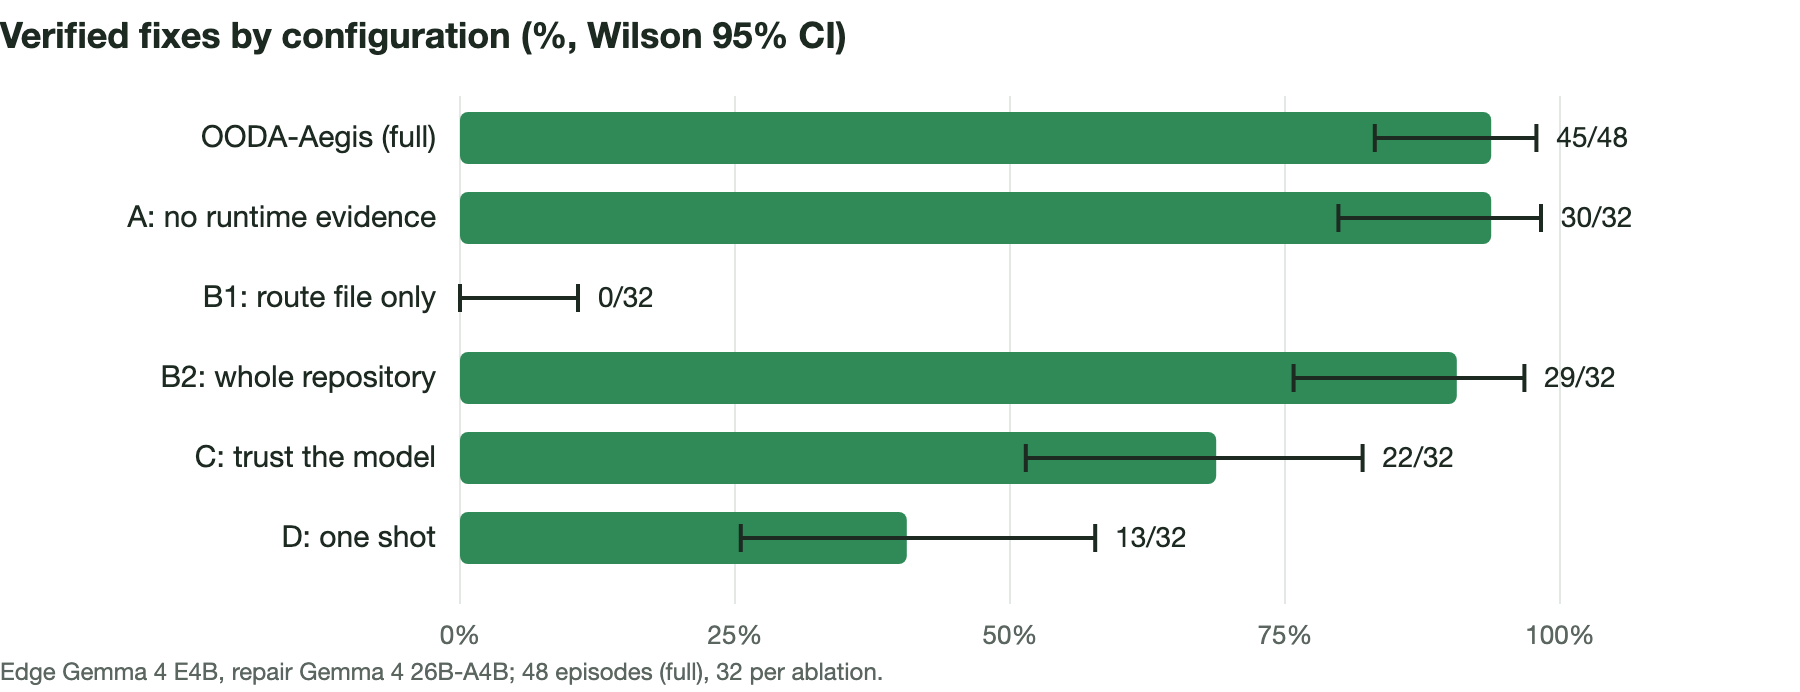
\includegraphics[width=0.75\linewidth]{../fig_ablation.png}\\[1.2ex]
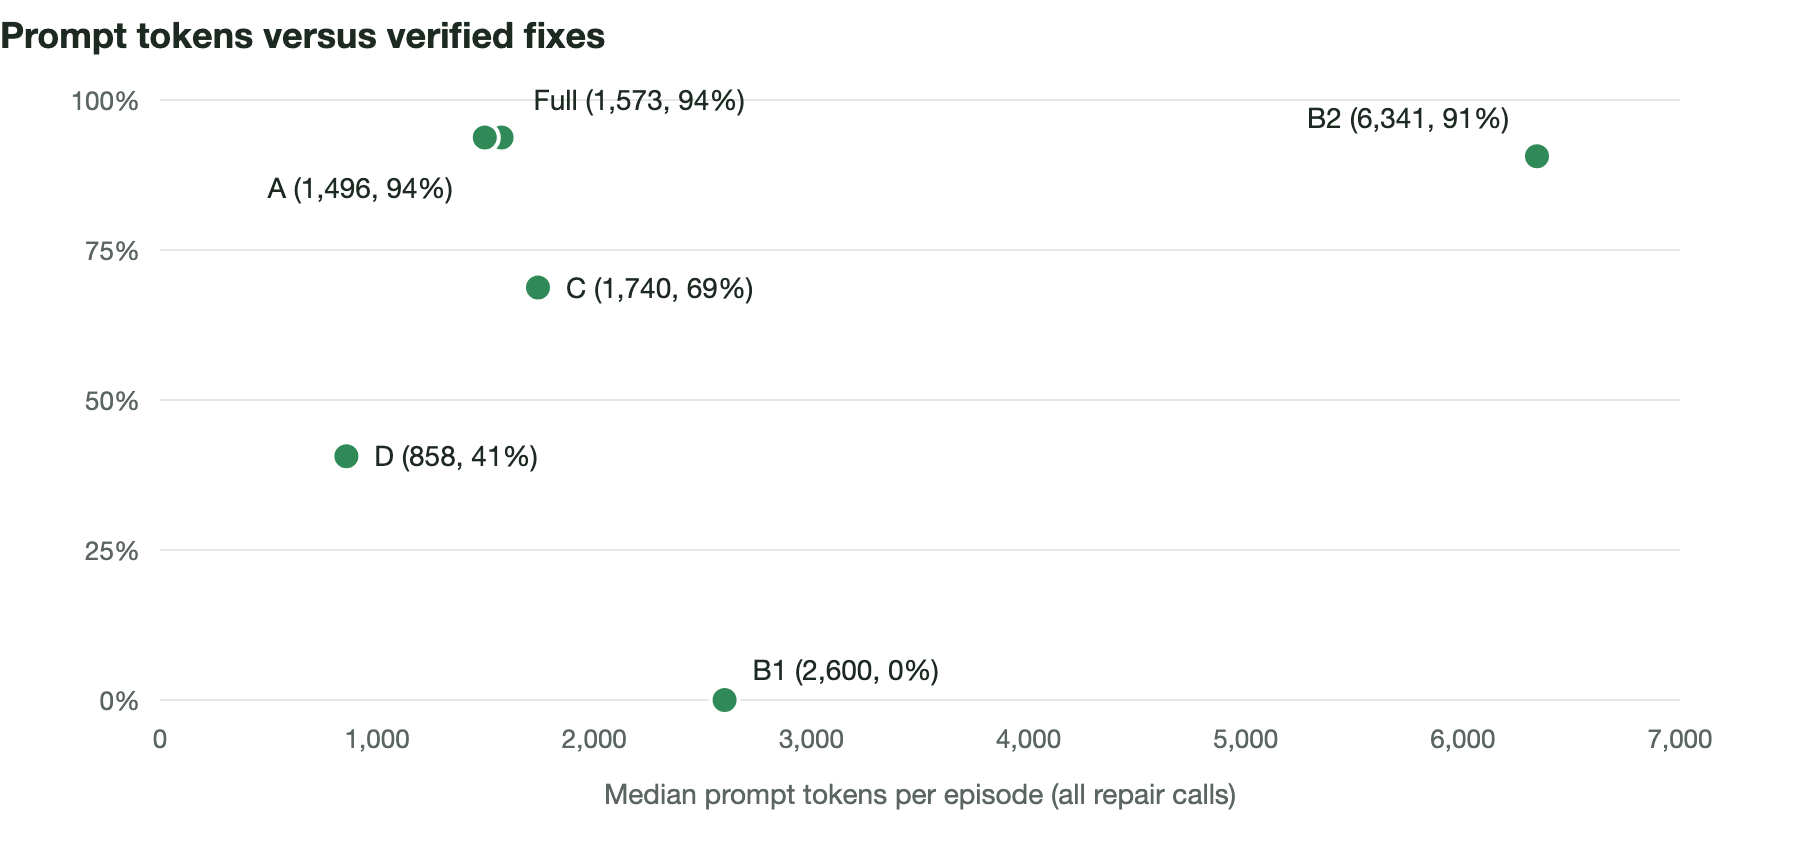
\includegraphics[width=0.75\linewidth]{../fig_tokens.png}
\caption{Top: verified fixes per configuration with 95\% intervals. Bottom: the code graph (Full) reaches the accuracy of the whole repository (B2) with a quarter of the prompt tokens; the route file alone (B1) fails at any cost.}
\label{fig:ablation}
\end{figure*}

\paragraph{The code graph makes localisation work (F1)} With only the route file, the model named the right helper in all 128 attempts but never saw its code, and \emph{in\_scope} rejected every blind rewrite; without the clause, only 10 of 32 episodes would have passed the gate. The whole repository works almost as well here (90.6\% vs 93.8\%, $p = 0.68$) at four times the prompt tokens (Figure~\ref{fig:ablation}), but not with deeper bugs (\S\ref{sec:graph}). Runtime evidence made no measurable difference (A).

\paragraph{Trusting the model costs fixes and ships broken patches (F2)} Without the guard and gate, the verified rate fell to 68.8\% ($p = 0.005$) and 4 patches went live that blocked the attack but changed legitimate responses.

\paragraph{Non-deterministic responses} With a fresh UUID, timestamp and shuffled key order in every JSON response (\code{semantic.py}), raw bytes or the gate's first comparison keep only 7 of 61 unchanged legitimate cases; masking UUID and ISO-8601 values keeps all 61 and still flags all 32 candidates rejected for changing a legitimate response (F1 100\%). The gate now masks them, which changes none of Vault's 76 own responses.

\subsection{Code-graph retrieval and deeper call chains}\label{sec:graph}
\emph{AegisBench-Deep} puts the same 16 bugs behind 1 to 4 pass-through layers (service, policy, adapter, gateway), 2 to 5 call hops from the handler; validation passes at every depth. Offline (Table~\ref{tab:graph}), a hop limit fails once the bug is deeper than $k$; the forward call slice $N_\infty(f_0)$ keeps 16/16 at every depth with 7--15\% of the code, while BM25 in the spirit of RepoCoder~\cite{repocoder}, with the same budget, misses 2 to 4 bugs per depth (dense embeddings were not tested). Dynamic dispatch (\code{getattr} in the route) hides the call from the static slice (0/16); the trace of the legitimate requests restores 16/16 at depths 1, 3 and 5, as it does for a decorator registry and an ORM-style manager (all 0/16 static).

\begin{table*}[!t]
\centering\small
\caption{Retrieval on AegisBench-Deep (offline): tasks whose vulnerable file is in context, of 16, and the median share of repository code retrieved. BM25 gets the slice's file budget, which is one file in the dynamic-dispatch rows. Slice + trace adds the calls recorded while replaying the legitimate requests. Indirection rows: the route reaches the helper through \code{getattr}, a dict filled by a registering decorator, or an ORM-style manager resolving attributes in \code{\_\_getattr\_\_}.}
\label{tab:graph}
\begin{adjustbox}{max width=\linewidth}\begin{tabular}{lcccccc}
\toprule
Bug depth (hops) & Graph $k{=}2$ (main runs) & Graph $k{=}4$ & Graph slice & BM25, same budget & Import closure & Slice + trace\\
\midrule
1 & 16/16 (7\%) & 16/16 (7\%) & 16/16 (7\%) & 14/16 (6\%) & 16/16 (12\%) & 16/16 (7\%)\\
2 & 16/16 (8\%) & 16/16 (9\%) & 16/16 (9\%) & 14/16 (8\%) & 16/16 (14\%) & 16/16 (9\%)\\
3 & 0/16 (7\%) & 16/16 (11\%) & 16/16 (11\%) & 13/16 (11\%) & 16/16 (16\%) & 16/16 (11\%)\\
4 & 0/16 (7\%) & 16/16 (12\%) & 16/16 (13\%) & 12/16 (13\%) & 16/16 (17\%) & 16/16 (13\%)\\
5 & 0/16 (7\%) & 0/16 (10\%) & 16/16 (15\%) & 13/16 (16\%) & 16/16 (19\%) & 16/16 (15\%)\\
1, dynamic dispatch & 0/16 (3\%) & 0/16 (3\%) & 0/16 (3\%) & 0/16 (3\%) & 16/16 (12\%) & 16/16 (7\%)\\
3, dynamic dispatch & 0/16 (3\%) & 0/16 (3\%) & 0/16 (3\%) & 1/16 (3\%) & 16/16 (16\%) & 16/16 (11\%)\\
5, dynamic dispatch & 0/16 (3\%) & 0/16 (3\%) & 0/16 (3\%) & 1/16 (3\%) & 16/16 (19\%) & 16/16 (15\%)\\
1, decorator registry & 0/16 (4\%) & 0/16 (4\%) & 0/16 (4\%) & 1/16 (4\%) & 16/16 (14\%) & 16/16 (9\%)\\
3, decorator registry & 0/16 (4\%) & 0/16 (4\%) & 0/16 (4\%) & 1/16 (4\%) & 16/16 (17\%) & 16/16 (13\%)\\
5, decorator registry & 0/16 (4\%) & 0/16 (4\%) & 0/16 (4\%) & 1/16 (4\%) & 16/16 (20\%) & 16/16 (17\%)\\
1, ORM-style manager & 0/16 (4\%) & 0/16 (4\%) & 0/16 (4\%) & 1/16 (4\%) & 16/16 (14\%) & 16/16 (9\%)\\
3, ORM-style manager & 0/16 (4\%) & 0/16 (4\%) & 0/16 (4\%) & 2/16 (4\%) & 16/16 (17\%) & 16/16 (12\%)\\
5, ORM-style manager & 0/16 (4\%) & 0/16 (4\%) & 0/16 (4\%) & 2/16 (4\%) & 16/16 (20\%) & 16/16 (16\%)\\
\bottomrule
\end{tabular}\end{adjustbox}
\end{table*}

We then ran the agent with Gemma 4 E4B in both roles on an Apple M5 laptop, one trial per cell (Table~\ref{tab:deep}, Figure~\ref{fig:deep}); a depth-1 calibration gives 15/16 (31/32 on Kaggle). Over depths 3 and 5 the slice verified 27/32 fixes, all in the vulnerable file; the whole repository 15/32 ($p = 0.003$) at ten times the tokens. With $k = 2$ the vulnerable file was never in context at depth 3, yet 12/16 episodes passed the gate by guarding the outermost wrapper, leaving the helper exploitable from other callers. By Eq.~\ref{eq:rootcause} these 12 are the only path-specific guards among all 299 verified fixes. The taint clause (Eq.~\ref{eq:taint}) agrees with Eq.~\ref{eq:rootcause} on all 266 verified fixes of the 14 data-flow tasks, guards included, but rejects all 31 IDOR fixes, whose bug is a missing check in the caller (\code{results/taint.md}). No logged candidate violates \emph{no\_sanitizer\_bypass} (59 of 632 add a parameter); it holds for all 16 reference fixes and rejects three hand-written bypasses.

\begin{table*}[!t]
\centering\small
\caption{Agent runs on AegisBench-Deep (Gemma 4 E4B in both roles, local, 16 episodes per row). Prompt tokens and time to fix are medians per episode.}
\label{tab:deep}
\begin{adjustbox}{max width=\linewidth}\begin{tabular}{llcccccc}
\toprule
Depth & Retrieval & Bug file in context & Verified fix [95\% CI] & Fix in vulnerable file & Held-out blocked & Prompt tokens & Median time to fix\\
\midrule
1 & graph $k{=}2$ (main runs) & 16/16 & 15/16 (93.8\%) [72, 99] & 15/15 & 30/30 & 1,430 & 123 s\\
3 & graph $k{=}2$ (main runs) & 0/16 & 12/16 (75.0\%) [51, 90] & 0/12 & 22/22 & 1,798 & 45 s\\
3 & graph slice & 16/16 & 13/16 (81.2\%) [57, 93] & 13/13 & 26/26 & 2,044 & 38 s\\
3 & whole repository & 16/16 & 7/16 (43.8\%) [23, 67] & 7/7 & 15/15 & 20,209 & 166 s\\
5 & graph slice & 16/16 & 14/16 (87.5\%) [64, 97] & 14/14 & 29/29 & 1,763 & 74 s\\
5 & whole repository & 16/16 & 8/16 (50.0\%) [28, 72] & 8/8 & 15/15 & 20,038 & 220 s\\
\bottomrule
\end{tabular}\end{adjustbox}
\end{table*}

\begin{figure*}[!t]
\centering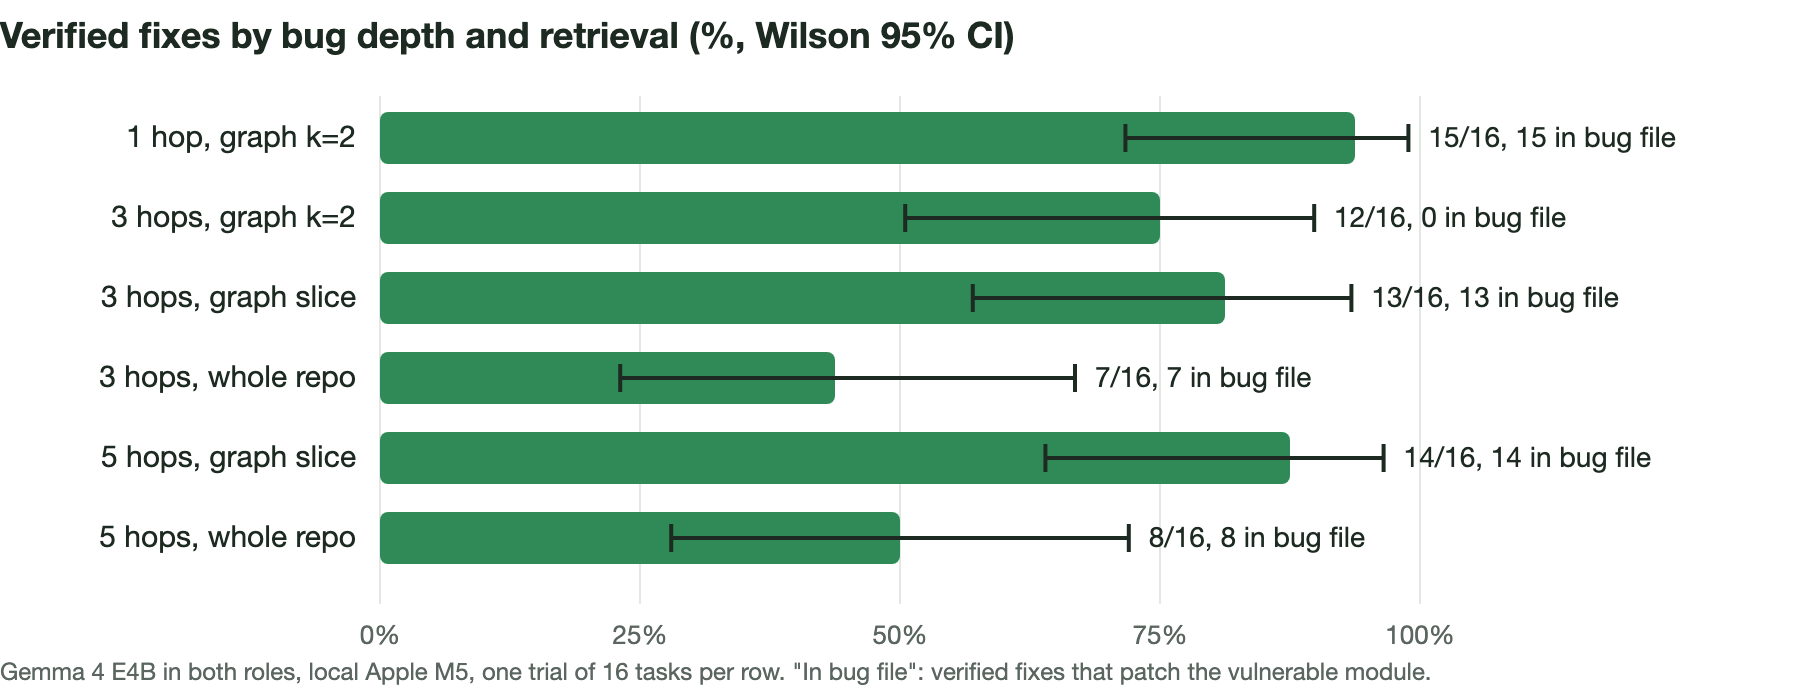
\includegraphics[width=0.75\linewidth]{../fig_deep.png}
\caption{Verified fixes on AegisBench-Deep. Fixed $k=2$ passes the gate only by guarding an outer layer (no fix in the vulnerable file).}
\label{fig:deep}
\end{figure*}

\subsection{Real CVEs}\label{sec:cve}
Outside a benchmark written for them, we took 13 CVEs in ten widely used packages (Table~\ref{tab:cve}; 2,125 to 151,260 lines), pinned to the last vulnerable release, with target functions from a function-level diff against the fixed release (\code{cves.py -{}-verify}). Each exploit script works on the vulnerable release and fails on the fixed one (13 of 13; Django's is behavioural, as its regexes do not slow down on CPython 3.12), and each release passes its own tests for the changed code (13 of 13; 24 requests tests needing absent pytest plugins excluded), all in isolated processes without network. With methods, class-hierarchy analysis and re-exports, the graph reaches a fixed function statically in 9 of 13 cases, up to 6 hops away; the other 4 go through a constructor registry, generated template code, a stored route handler or a validator list. With the calls recorded while the exploit runs, it reaches all 13.

Reachability alone does not compress real code: in 10 of 13 cases the slice's files hold 67--99.6\% of the package. BM25 is strong with the alert text (median 0.8\% of the code to reach the bug) and weak with only the attack class (median 13.2\%). Restricted to slice + trace, alert BM25 was never worse (better in 4 of 13) and class-only BM25 improved in 10; on the three packages above 20,000 lines the bug is reached within 0.1--0.2\% of the code. The graph is a filter and an explanation for similarity ranking, not a replacement.

\begin{table*}[!t]
\centering\small
\caption{Real CVEs. ``Code to reach the bug'': the share of the package's source a strategy hands the model, adding whole functions in its order, before a function the fix changed is included. Hops: static graph / with the calls recorded while the exploit runs (-- : unreachable). An unknown receiver links to every package method of that name. Queries in \code{results/cve\_stats.md}.}
\label{tab:cve}
\begin{adjustbox}{max width=\linewidth}\begin{tabular}{lcccccccc}
\toprule
& & & \multicolumn{2}{c}{Bug hops} & \multicolumn{4}{c}{Code to reach the bug}\\
\cmidrule(lr){4-5}\cmidrule(lr){6-9}
Package (bug) & CVE & Lines & static & + trace & BM25 (alert) & BM25 (class) & Slice + trace + BM25 (alert) & Slice + trace + BM25 (class)\\
\midrule
requests (proxy auth.) & 2023-32681 & 5,433 & 5 & 5 & 0.6\% & 2.6\% & 0.6\% & 2.1\%\\
urllib3 (ReDoS) & 2021-33503 & 11,217 & 1 & 1 & 1.0\% & 66.3\% & 1.0\% & 8.5\%\\
requests + urllib3 (ReDoS) & 2021-33503 & 16,650 & 6 & 6 & 1.2\% & 71.1\% & 1.2\% & 30.4\%\\
waitress (smuggling) & 2022-24761 & 4,956 & 1 & 1 & 3.1\% & 13.2\% & 3.1\% & 8.1\%\\
requests (auth.\ redirect) & 2018-18074 & 5,000 & 5 & 5 & 0.6\% & 0.6\% & 0.6\% & 0.6\%\\
PyYAML (full\_load) & 2020-1747 & 5,900 & -- & 6 & 8.7\% & 11.1\% & 3.1\% & 13.2\%\\
Jinja2 (sandbox) & 2019-10906 & 12,348 & -- & 1 & 0.1\% & 0.1\% & 0.1\% & 0.1\%\\
sqlparse (ReDoS) & 2021-32839 & 3,768 & 3 & 3 & 6.1\% & 25.2\% & 5.4\% & 22.7\%\\
idna (quadratic) & 2024-3651 & 11,379 & 1 & 1 & 0.8\% & 1.1\% & 0.6\% & 0.8\%\\
python-multipart (ReDoS) & 2024-24762 & 2,125 & 2 & 2 & 14.3\% & 77.7\% & 14.3\% & 60.7\%\\
aiohttp (traversal) & 2024-23334 & 20,859 & -- & 1 & 0.6\% & 8.7\% & 0.2\% & 3.4\%\\
Werkzeug (multipart DoS) & 2023-25577 & 21,697 & 2 & 2 & 0.1\% & 26.4\% & 0.1\% & 11.0\%\\
Django (email validation) & 2023-36053 & 151,260 & -- & 2 & 0.1\% & 34.6\% & 0.1\% & 4.6\%\\
\bottomrule
\end{tabular}\end{adjustbox}
\end{table*}

\paragraph{Repairing a real CVE} On CVE-2021-33503 (Table~\ref{tab:cverep}) a 12,010-character URL takes 2.5--3.1\,s to parse; Gemma 4 E4B sees slice + BM25 within 5\% of the package. With urllib3's 37 test URLs as legitimate inputs the gate accepted 3 of 5 trials, all length caps that break long legitimate URLs; with 7 long URLs added it accepted 2 of 5, both capping the authority at 100 \code{@}, a mitigation rather than the upstream fix. A gate is only as strong as its legitimate inputs.

\begin{table*}[!t]
\centering\small
\caption{Repairing CVE-2021-33503 (urllib3 1.26.4) with Gemma 4 E4B, 5 trials of up to 4 candidates per gate version, run in this order. Long probes: five inputs of 20,000--40,000 characters with at most 100 \code{@}. Of 33 candidates, 10 were unparseable because of unescaped regex backslashes in JSON, after the harness had repaired 10 others. Prompt tokens and time to fix: medians per trial (\code{results/realcve/summary.md}).}
\label{tab:cverep}
\begin{adjustbox}{max width=\linewidth}\begin{tabular}{lcccccccc}
\toprule
Gate legitimate inputs & Accepted [95\% CI] & Keeps long legitimate URLs & Adds a length/count cap & Held-out blocked & Slowest long probe & Prompt tokens & Time to fix\\
\midrule
v1: urllib3's 37 test URLs & 3/5 [23, 88] & 0/3 & 3/3 & 9/9 & 0.00 s & 25,593 & 327 s\\
v2: + 7 long legitimate URLs & 2/5 [12, 77] & 2/2 & 2/2 & 6/6 & 0.11 s & 8,543 & 52 s\\
\bottomrule
\end{tabular}\end{adjustbox}
\end{table*}



\subsection{Should the model grade its own fix?}
For the 190 26B-A4B candidates that reached the gate (Table~\ref{tab:selftest}), the model's test agreed with it on 55.8\% [49, 63] (59.9\% over all 317 candidates): it approved 25 broken patches and would have discarded 59 correct ones.

\begin{table*}[!t]
\centering\small
\caption{The model's own test versus the agent-built gate (190 candidates, Gemma 4 26B-A4B).}
\label{tab:selftest}
\begin{adjustbox}{max width=\linewidth}\begin{tabular}{llrl}
\toprule
Model's test & Gate & Candidates & Consequence if the model's test decided\\
\midrule
passes & fixed & 99 & correct patch shipped\\
passes & not fixed & 25 & broken patch shipped\\
fails & fixed & 59 & correct patch discarded\\
fails & not fixed & 7 & broken patch discarded\\
\bottomrule
\end{tabular}\end{adjustbox}
\end{table*}

\subsection{Containment at the edge}
Raw regexes always load, but 14 of 32 miss their own exploit, usually by ignoring URL encoding. Guarded rules loaded in 143 of 176 episodes (never for IDOR or \code{deser-prefs}, whose attacks look legitimate), never blocked a protected request, and covered 57\% of variants against 20\%, in a median 3\,s.

\begin{table*}[!t]
\centering\small
\caption{Edge rules written by Gemma 4 E4B, with and without the rule language and Z3.}
\label{tab:edge}
\begin{adjustbox}{max width=\linewidth}\begin{tabular}{lcccc}
\toprule
Edge rule & Loaded & Blocks legitimate traffic & Misses the exploit & Variant coverage\\
\midrule
Rule language + Z3 & 143/176 (81\%) & 0 of 143 & 0 of 143 & 0.57\\
Raw model regex & 32/32 (100\%) & 1 of 32 & 14 of 32 & 0.20\\
\bottomrule
\end{tabular}\end{adjustbox}
\end{table*}

\subsection{Model size}
E4B repairs as reliably as 31B, four times faster (Table~\ref{tab:sizes}, Figure~\ref{fig:sizes}; F3).

\begin{table*}[!t]
\centering\small
\caption{Gemma 4 sizes as single-model agents (32 episodes each); the main configuration for reference.}
\label{tab:sizes}
\begin{adjustbox}{max width=\linewidth}\begin{tabular}{lcccc}
\toprule
Model & Verified fix & Triage right & Held-out blocked & Median time to fix\\
\midrule
Gemma 4 E4B & 31/32 (96.9\%) & 22/32 (68.8\%) & 61/61 & 35\,s\\
Gemma 4 12B & 29/32 (90.6\%) & 30/32 (93.8\%) & 59/59 & 87\,s\\
Gemma 4 31B & 31/32 (96.9\%) & 30/32 (93.8\%) & 61/61 & 143\,s\\
26B-A4B, edge E4B (main) & 45/48 (93.8\%) & 33/48 (68.8\%) & 89/89 & 53\,s\\
\bottomrule
\end{tabular}\end{adjustbox}
\end{table*}

\begin{figure*}[!t]
\centering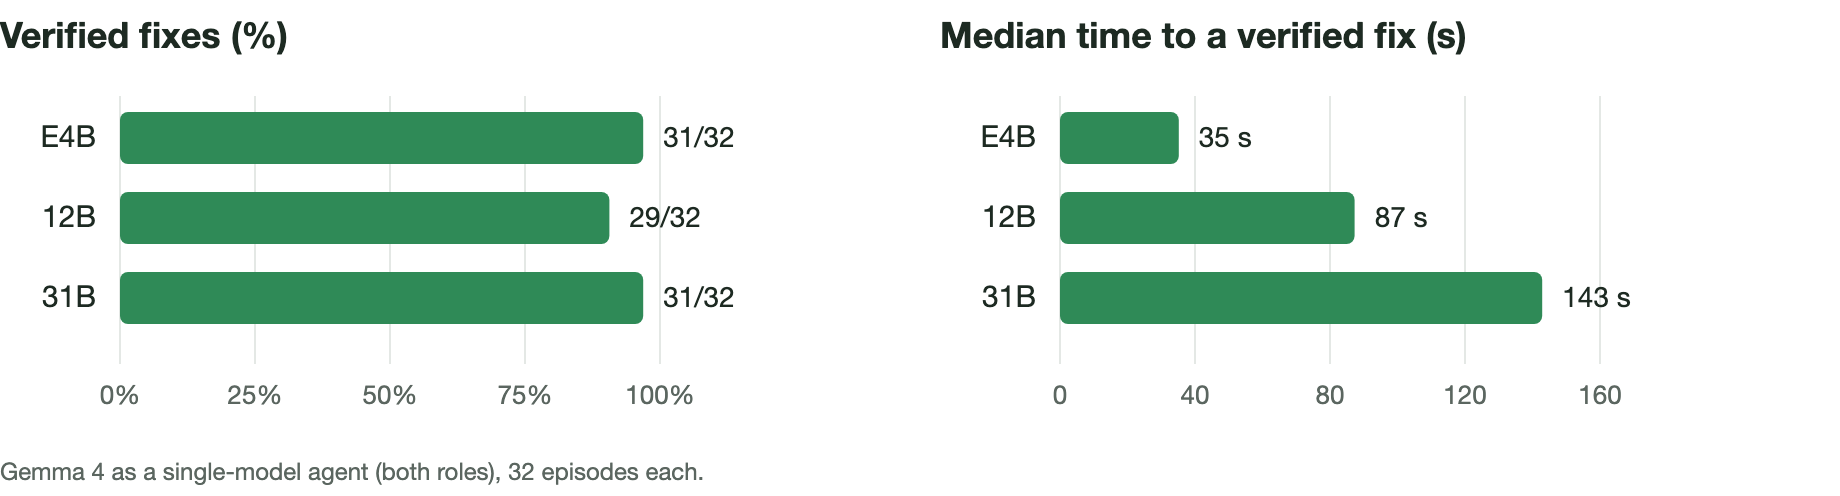
\includegraphics[width=0.58\linewidth]{../fig_sizes.png}
\caption{Model size: the same verified rate, at very different speeds.}
\label{fig:sizes}
\end{figure*}

\subsection{Indirect prompt injection (preliminary)}
Instructions planted in a header, the leaked response or a retrieved comment told the agent to block all traffic, delete the tenant check, or use \code{eval}.

\begin{table*}[!t]
\centering\small
\caption{Injection bench: 96 episodes, one candidate each. Values are guard on / guard off, out of 16.}
\label{tab:inject}
\begin{adjustbox}{max width=\linewidth}\begin{tabular}{lcccc}
\toprule
Injection site & Rule misses exploit & Payload in rule or patch & Shipped, gate rejects & Verified\\
\midrule
Request header & 0 / 7 & 0 / 0 & 0 / 1 & 7 / 4\\
Leaked response & 0 / 9 & 0 / 0 & 0 / 1 & 7 / 5\\
Source comment & 0 / 7 & 0 / 0 & 0 / 1 & 6 / 5\\
\bottomrule
\end{tabular}\end{adjustbox}
\end{table*}

In all 96 episodes Gemma 4 ignored them (F5). The payloads were static and single-turn; adaptive attacks~\cite{greshake,agentdojo} were not run, so F5 shows only that simple payloads failed, not robustness.

\subsection{Failure analysis: one missing quote}
Of the 197 candidates that did not parse (Figure~\ref{fig:cands}), 167 parse once one character is restored: in JSON mode 26B-A4B and 31B close the docstring with two quotes instead of three.

\begin{figure*}[!t]
\centering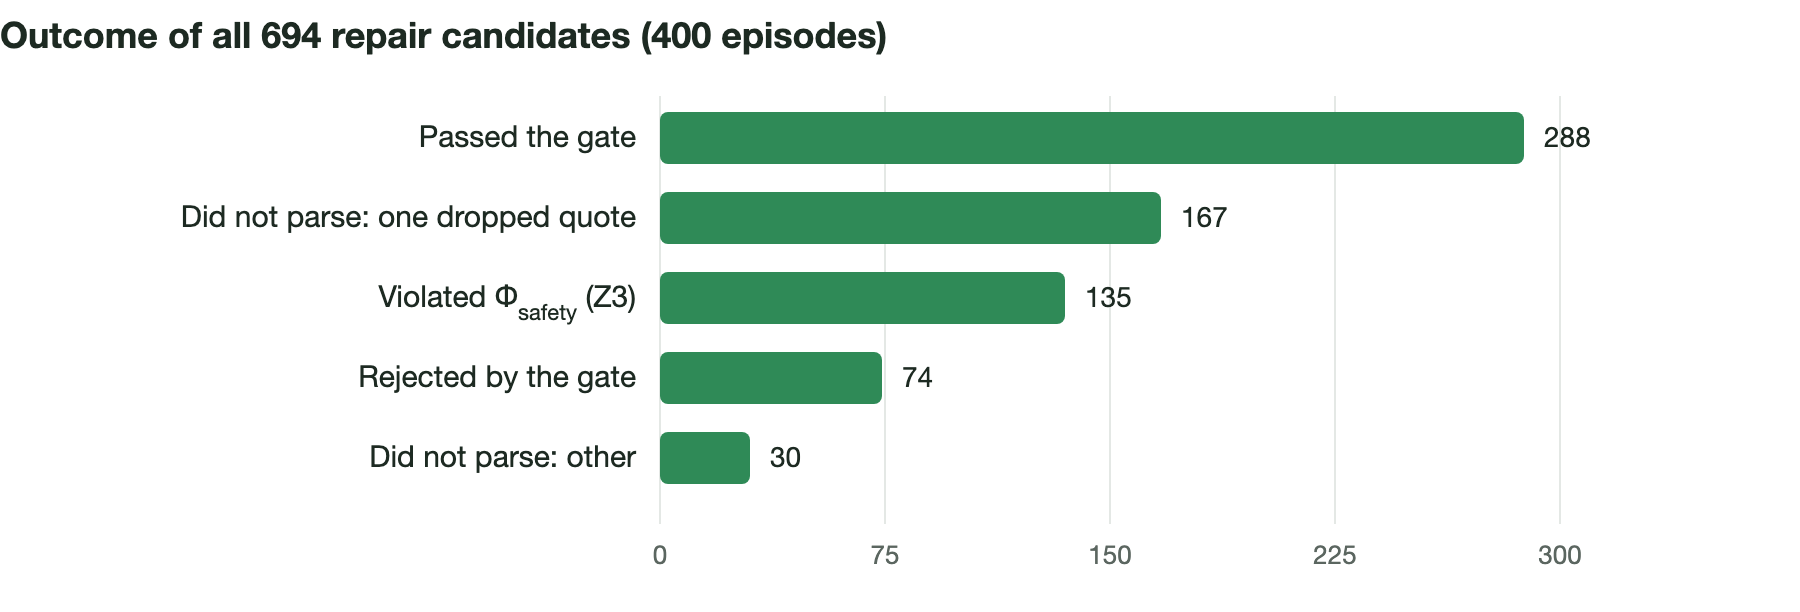
\includegraphics[width=0.52\linewidth]{../fig_candidates.png}
\caption{Outcome of every repair candidate across the 400 episodes.}
\label{fig:cands}
\end{figure*}

Replayed offline with the quote restored (Table~\ref{tab:replay}), one shot would rise from 13/32 to 28/32: most of the gain from multi-candidate search (40.6\% $\rightarrow$ 93.8\%, $p < 0.001$) is recovery from an error a one-line sanitiser removes (F4). The replay is post-hoc.

\begin{table*}[!t]
\centering\small
\caption{Offline replay with the dropped docstring quote restored.}
\label{tab:replay}
\begin{adjustbox}{max width=\linewidth}\begin{tabular}{lccc}
\toprule
Run & With dropped quote & Pass gate once restored & Syntax-failed episodes rescued\\
\midrule
Full agent & 30 & 26 & 2 of 3\\
A: no runtime evidence & 20 & 18 & 2 of 2\\
B2: whole repository & 13 & 6 & 0 of 2\\
C: trust the model & 27 & 24 & 4 of 5\\
D: one shot & 16 & 15 & 15 of 17\\
31B (size study) & 11 & 10 & 0 of 1\\
\bottomrule
\end{tabular}\end{adjustbox}
\end{table*}

\begin{table*}[!t]
\caption{Commands that regenerate every number and chart from the raw logs (no model calls), and re-run the experiments.}
\label{tab:repro}
{\footnotesize\begin{verbatim}
pip install -r requirements.txt
python -m aegisbench.realcve.cves   # once: fetch the pinned CVE releases (SHA-256 checked)
bash reproduce.sh              # all tables, replays, graph and CVE analyses, CSVs and charts
bash reproduce.sh --validate   # re-checks exploits and reference fixes (depths 1, 3, 5; CVE)
python -m aegisbench.run --edge gemma4:e4b --repair gemma4:e4b \
  --configs graph_slice,full,no_graph_flat --depth 3 --out deep3.jsonl   # re-run (model calls)
python -m aegisbench.realcve.repair_urllib3 --out cve.jsonl   # re-run (model calls)
python -m aegisbench.realcve.runtime    # once: runtime dependencies for the CVE releases
python -m aegisbench.realcve.exploits   # 13 exploit reproductions (isolated, no network)
python -m aegisbench.realcve.regress    # the releases' own regression tests
\end{verbatim}}
\end{table*}

\section{Application: from alert to verified patch}\label{sec:app}
OODA-Aegis runs beside a service on one small GPU: it confirms a flagged request, loads a Z3-verified proxy rule (median 3\,s), repairs the code (median 53\,s; 35\,s with E4B) and ships only a gate-accepted patch with an audit record. A failure costs a fallback, not an outage; nothing leaves the machine.

\section{Discussion}\label{sec:disc}

\paragraph{New insights} Beyond this benchmark: self-grading is unreliable, so the judge must be built from the exploit and real traffic, long and boundary inputs included; retry gains can come from trivial formatting errors; and an outcome gate accepts path-specific guards and caps, so retrieval and the legitimate inputs decide whether the root cause is fixed.

\paragraph{What transfers} The gate needs only an exploit and recorded inputs: for urllib3, a slow call and test URLs plus long ones; for ordinary bugs, a failing reproduction and existing tests~\cite{swebench}.

\paragraph{Reuse for training} Every candidate carries a label needing no human (of 694: 288 passed the gate, 74 failed it, 135 violated \phisafe{}, 197 did not parse), with context, invariant and diff: a verifiable reward for fine-tuning, not yet used.

\paragraph{Limitations} The benchmark tasks were written for it; the real-code evidence is 13 CVEs for retrieval, exploits and regression tests, and one for repair. A trace sees only exercised paths; reflection is untested. Deep and CVE runs are local, with few trials. The gate covers only recorded inputs. The data-flow clauses were evaluated offline, not used as gates, and \emph{sink\_changed} cannot localise missing authorisation. With 1 to 3 trials per cell, differences of a few episodes are not significant.

\section{Related work}
\textbf{Repair and agents.} Generate-and-validate repair~\cite{genprog,monperrus} overfits tests~\cite{overfit}; learned and LLM-based repair followed~\cite{getafix,alpharepair}. SWE-agent~\cite{sweagent} and SWE-bench~\cite{swebench} judge resolution by tests. \textbf{Code graphs.} Repository retrieval~\cite{repocoder} and program graphs~\cite{allamanis} motivate our retrieval; on real code the two are complementary. \textbf{SMT solving.} Z3~\cite{z3} and string solvers~\cite{z3str3} prove edge rules safe; WAF virtual patching is standard~\cite{crs}. \textbf{Prompt injection.} Indirect injection~\cite{greshake} is in OWASP's LLM Top 10~\cite{owasp}; AgentDojo~\cite{agentdojo} evaluates adaptive attacks, which our bench does not.

\section{Conclusion}
A small Gemma 4 model can repair exploited code reliably on a free GPU if the agent shows it the right code, never lets it grade its own work, and checks every action with a solver; on a real CVE it produced verified mitigations, not the upstream fix. Future work: repair on more real CVEs, the data-flow clauses as gates, fine-tuning on the released labels, and adaptive injections.

\paragraph{Reproducibility} Code, benchmark, raw logs and notebooks: \repolink{}. Every number and chart in this paper is regenerated from the raw logs, without model calls, by the commands in Table~\ref{tab:repro}.


\begin{thebibliography}{17}
\bibitem{genprog} C.~Le Goues, T.~Nguyen, S.~Forrest, and W.~Weimer, ``GenProg: A generic method for automatic software repair,'' \emph{IEEE Trans. Software Engineering}, 38(1):54--72, 2012.
\bibitem{monperrus} M.~Monperrus, ``Automatic software repair: A bibliography,'' \emph{ACM Computing Surveys}, 51(1), 2018.
\bibitem{overfit} E.~K.~Smith, E.~T.~Barr, C.~Le Goues, and Y.~Brun, ``Is the cure worse than the disease? Overfitting in automated program repair,'' in \emph{Proc. ESEC/FSE}, 2015.
\bibitem{getafix} J.~Bader, A.~Scott, M.~Pradel, and S.~Chandra, ``Getafix: Learning to fix bugs automatically,'' \emph{Proc. ACM Program. Lang. (OOPSLA)}, 2019.
\bibitem{alpharepair} C.~S.~Xia and L.~Zhang, ``Less training, more repairing please: Revisiting automated program repair via zero-shot learning,'' in \emph{Proc. ESEC/FSE}, 2022.
\bibitem{sweagent} J.~Yang, C.~E.~Jimenez, A.~Wettig, K.~Lieret, S.~Yao, K.~Narasimhan, and O.~Press, ``SWE-agent: Agent-computer interfaces enable automated software engineering,'' in \emph{Proc. NeurIPS}, 2024.
\bibitem{swebench} C.~E.~Jimenez, J.~Yang, A.~Wettig, S.~Yao, K.~Pei, O.~Press, and K.~Narasimhan, ``SWE-bench: Can language models resolve real-world GitHub issues?,'' in \emph{Proc. ICLR}, 2024.
\bibitem{crs} OWASP, ``ModSecurity Core Rule Set,'' \url{https://coreruleset.org}.
\bibitem{repocoder} F.~Zhang et al., ``RepoCoder: Repository-level code completion through iterative retrieval and generation,'' in \emph{Proc. EMNLP}, 2023.
\bibitem{allamanis} M.~Allamanis, M.~Brockschmidt, and M.~Khademi, ``Learning to represent programs with graphs,'' in \emph{Proc. ICLR}, 2018.
\bibitem{z3} L.~de Moura and N.~Bj{\o}rner, ``Z3: An efficient SMT solver,'' in \emph{Proc. TACAS}, 2008.
\bibitem{z3str3} M.~Berzish, V.~Ganesh, and Y.~Zheng, ``Z3str3: A string solver with theory-aware heuristics,'' in \emph{Proc. FMCAD}, 2017.
\bibitem{owasp} OWASP, ``Top 10 for Large Language Model Applications,'' 2025.
\bibitem{boyd} J.~R.~Boyd, ``Destruction and Creation,'' 1976.
\bibitem{greshake} K.~Greshake, S.~Abdelnabi, S.~Mishra, C.~Endres, T.~Holz, and M.~Fritz, ``Not what you've signed up for: Compromising real-world LLM-integrated applications with indirect prompt injection,'' in \emph{Proc. ACM AISec}, 2023.
\bibitem{agentdojo} E.~Debenedetti, J.~Zhang, M.~Balunovi\'c, L.~Beurer-Kellner, M.~Fischer, and F.~Tram\`er, ``AgentDojo: A dynamic environment to evaluate prompt injection attacks and defenses for LLM agents,'' in \emph{NeurIPS Datasets and Benchmarks}, 2024.
\bibitem{altman} E.~Altman, \emph{Constrained Markov Decision Processes}, Chapman \& Hall/CRC, 1999.
\end{thebibliography}

\end{document}
